%@@@@@@@@@@@@@@@@@@@@@@@@@@@@@@@@@@@@@@@@@@@@@@@@@@
\chapter{RVQ (Residual Vector Quantization)}
\label{chap_RVQ}	
%@@@@@@@@@@@@@@@@@@@@@@@@@@@@@@@@@@@@@@@@@@@@@@@@@@

\begin{figure}[htp]			
	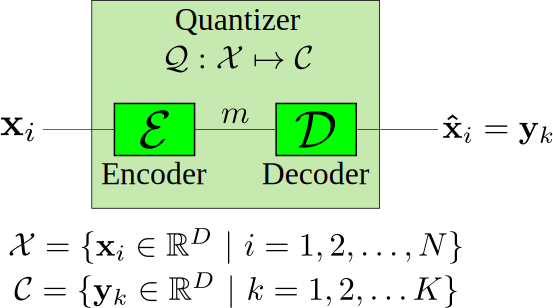
\includegraphics[width=1\textwidth]{thesis/Quantization_blockDiagram.pdf}
	\caption{A quantizer $Q$ maps symbols from a source alphabet $\mathcal{X}$ to symbols from a reconstruction alphabet $\mathcal{C}$, where in general, the number of elements in $\mathcal{C}$, $|\mathcal{C}| << |\mathcal{X}|$, the number of elements in $\mathcal{X}$ }
	\label{fig:Quantization_block_diagram}
\end{figure}

%####################
\section{Quantization}
%####################
%====================
\subsection{Introduction}
\label{sec:quantization}
%====================

The main mechanism for achieving lossy compression in images and videos is the process of \emph{quantization}.  For instance, all current video standards, MPEG-1, MPEG-2, MPEG-4, H.261, H.263 and H.264 rely on a special form quantization called \emph{transform vector quantization}, for compression.  Quantization is the process of representing a large, possibly infinite, set of values with a smaller set of values.  Figure~\ref{fig:Quantization_block_diagram} shows a quantizer $Q$ that takes values from a source alphabet $\mathcal{X}$,

\begin{equation}
\mathcal{X}=\{x \in \mathcal{R}^D\}
\end{equation}

and maps them to a reconstruction alphabet $\mathcal{C}$, 

\begin{equation}
\mathcal{C}=\{\mu_k \in \mathcal{R}^D | k=1,2, \ldots K\}
\end{equation}

The $K$ partitions $P_k, k = 1, 2, \ldots, K$ created in the input space $R^D$, 

\begin{equation}
P_k = \{x \in R^D | Q(x) = \mu_k\}
\end{equation}   

are mutually exclusive,

\begin{equation}
P_i \bigcap P_j = \emptyset, \ i \neq j
\end{equation}

and the union of these partitions covers the entire input space,

\begin{equation}
\bigcup\limits_{k=1}^{K} P_k=\mathcal{R}^D
\end{equation}

The reconstruction alphabet is also known as the \emph{codebook}.  Members of this set, $\mu_k$ are called \emph{codevectors}.  If the input is scalar, i.e. $D=1$, the quantizer is called a \emph{scalar quantizer} (SQ).  For $D>1$, the quantizer is called a \emph{vector quantizer} (VQ).  The \emph{resolution}, \emph{code rate}, or simply the \emph{rate} $r$ of a quantizer, 


\begin{figure}[t]			
	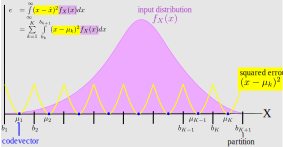
\includegraphics[width=1\textwidth]{thesis/Quantization_MSE.pdf}
	\caption{Computing optimal centroids.}
	\label{fig:computing_optimal_centroids}	
\end{figure}

\begin{equation}
r=\frac{\log_2 K}{D}
\end{equation}  

is proportional to the number of bits required to represent the total number of codevectors, $K$ and inversely proportional to the dimensionality of the data.  This shows that for the same number of codevectors $K$, the rate increases linearly with the dimensionality of the data.  VQ is therefore able to achieve higher rates than SQ.  However, for a given error metric $d(.)$, a common one being the squared error criterion, 

\begin{equation}
d(x,y)=(x-y)^2 
\end{equation}

higher rates can increase distortion $\mathcal{D}$,

\begin{equation}
\mathcal{D(\mathcal{X}, \mathcal{C})} =E\left[d(x, Q(x)) \right]
\end{equation}

This tradeoff between rate and distortion can be plotted to create a \emph{rate-distortion} curve.  A fundamental result of Shannon's rate-distortion theory is that VQ will always achieve equal better or equal compression rates than SQ, even if the source is memoryless, i.e., emits a sequence of IID random variables \cite{1984_JNL_VQ_Gray}.   The reason is that SQ quantizes each dimension separately and cannot therefore exploit statistical correlation between the different dimensions of the data.  The result is rectangular partitions $P_k$ in $R^D$.  On the other hand, VQ can carve up the input space into arbitrary shapes.

\begin{figure}[t]		
	\center	
	\includegraphics[height=0.4\textheight]{thesis/MPEG4_VTK.png}
	\caption{Scalar quantization in the transform domain for MPEG-4.  The image on the left shows the 3 intensity channels of an input image patch drawn in the YUV color space.  The vertical dimension is the luma (Y) axis.  The right image shows the quantized reconstruction of the input image patch.  No deblocking filter has been used, and so the loss of information is entirely due to quantization.  Notice the straight lines along which the output pixels are aligned due to the quantization process.  The visualization was created using the Visualization Toolkit (VTK) \cite{VTK} in C.}
	\label{fig:MPEG4_VTK}
\end{figure}


%====================
\subsection{Optimality issues}
%====================
\begin{figure}[t]		
	\center	
	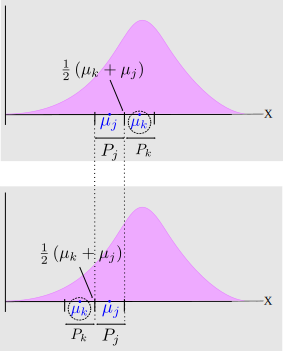
\includegraphics[height=0.5\textheight]{thesis/Quantization_optimalPartitions2.pdf}
	\caption{Computing optimal partitions}
	\label{fig:computing_optimal_partitions}
\end{figure}

So far, no mention has been made about optimality of the codevectors or partitions.  A widely used algorithm to compute optimal codevectors and partitions is the Generalized Lloyd Algorithm (GLA) \cite{1991_BOOK_VQ_GershoGray}, also known as the Linde Buzo Gray (LBG) algorithm \cite{1982_JNL_LeastSquaresQuantization_Lloyd} or K-means clustering \cite{1967_CNF_Kmeans_Macqueen}.  Figure~\ref{fig:computing_optimal_centroids} illustrates the SQ case for an input $X$ with distribution $f_X(x)$ and squared error criterion, 

\begin{equation}
e=\sum\limits_{k=1}^{N} \int\limits_{b_k}^{b_{k+1}}(x-\mu_k)^2f_X(x)
\end{equation}

If the partitions $P_k$,

\begin{equation}
\label{Eq:partitions}
P_k =  \left\{x \ | \ (\mu_j-x)^2 < (\mu_k-x)^2, \ \forall \ j \neq k \right\}
\end{equation}

are given, an optimal codevector $\mu_k$ can be computed by setting the derivative of the error $e$ with respect to $\mu_k$ equal to 0,

\begin{equation}
\frac{\partial{e}}{\partial{\mu_k}} = 0
\end{equation}

In other words, the optimal centroid for a given partition and the squared error criterion is the centroid of the partition. 

\begin{equation}
\mu_k = \frac
{\int\limits_{b_k}^{b_{k+1}}xf_X(x)dx}
{\int\limits_{b_k}^{b_{k+1}}f_X(x)dx}
\end{equation}

To compute optimal partitions, given the centroids, we can rewrite Equation~\ref{Eq:partitions} as 

\begin{equation}
\label{Eq:partitions2}
P_j=\left\{x \ | \ (\mu_k -\mu_j) \left(x - \frac{1}{2} \left(\mu_k + \mu_j \right)\right) < 0, \ \forall j \neq k 
\right\}
\end{equation}

For the scalar case in Figure~\ref{fig:computing_optimal_partitions}, if $k>j$, i.e. $(\mu_k -\mu_j) > 0$, then to satisfy Equation~\ref{Eq:partitions2}

\begin{align}
\label{Eq:partitions3}
x - \frac{1}{2} \left(\mu_k + \mu_j \right) &< 0\notag\\
\Rightarrow x &< \frac{1}{2} \left(\mu_k + \mu_j \right)
\end{align}

Conversely, if $k<j$, i.e. $(\mu_k -\mu_j) < 0$, then to satisfy Equation~\ref{Eq:partitions2}

\begin{align}
\label{Eq:partitions4}
x - \frac{1}{2} \left(\mu_k + \mu_j \right) &> 0 \notag\\
\Rightarrow x &> \frac{1}{2} \left(\mu_k + \mu_j \right)
\end{align}

The only way to satisfy both Equations~\ref{Eq:partitions3} and \ref{Eq:partitions4} is for the partition boundary to be half-way between the centroids, , i.e. $\frac{1}{2} \left(\mu_k + \mu_j \right)$.  This notion can be generalized to the vector case.

%=================
\subsection{Types of VQ}
%=================
\begin{figure}[htp]				
	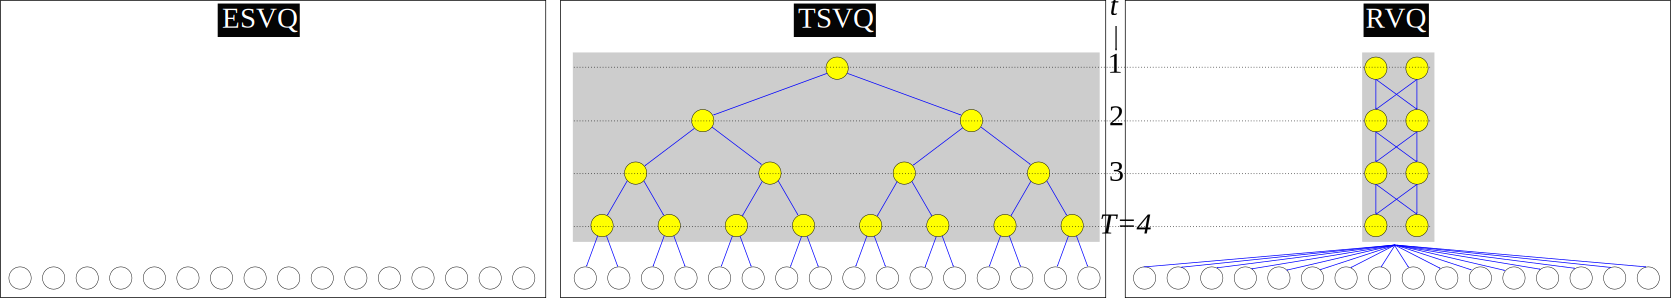
\includegraphics[width=1.1\textwidth]{thesis/RVQ_comparisonWithESVQ_TSVQ.pdf}
	\caption{Graphical comparison of ESVQ, TSVQ and RVQ, 16 codevectors}
	\label{fig:comparison_ESVQ_TSVQ_RVQ}
\end{figure}

\begin{table}[htp]
\begin{longtable}{| p{2.2in} || p{1in} | p{1.5in} | p{1.5in}|}
\hline
											&ESVQ						&TSVQ																&RVQ								\\ 
\hline
\# data points								&$N$						&same																&same								\\ 
\hline
Vertical dimension, $T$					&-							&depth																&\# stages							\\
Horizontal dimension, $M$					&-							&breadth															&\# templates						\\
Encoding indeces							&-							&path map	(T-tuple)												&XDR (T-tuple)						\\ 
\hline
Input dimension							&$D$						&same																&same								\\
Rate, $r$ (bits/vector component)			&$(\log_2K)/D$			&same																&same								\\ 
\hline
\# non-terminal codevectors, $N_{ntc}$	&0							&$1+M+M^2+ \ldots + M^{T-1}=\frac{M^T-1}{M-1}$			&$MT$								\\
\# terminal codevectors, $K$				&$2^{rD}$					&$2^{rD}=M^T$													&same as TSVQ					\\
\hline
computations: search ops/stage			&1 stage, $O(2^{rD})$	&$M$																&same as TSVQ					\\
computations: search complexity 			&$O(2^{rD})$				&O($MT$)															&same  as TSVQ					\\ 
memory 									&$2^{rD}$					&$MN_{ntc} = M\frac{M^T-1}{M-1}\approx\frac{M}{M-1}M^T$ &$MT$								\\ 
\hline
\# Input data at stage $t$					&1 stage, $N$				&$\frac{N}{M^t}$													&$N$								\\
\hline
\end{longtable}
\caption{Comparison of ESVQ, TSVQ and RVQ}
\label{tab:comparison_ESVQ_TSVQ_RVQ}
\end{table}
We now list the main types of VQ that appear in the literature.  The goal of VQ design is to have output distortion as close as possible to the rate-distortion curve.  However, in general, optimal coding of source vectors is not possible unless an exhaustive search over all code-vectors is carried out, as in structurally unconstrained \emph{Exhaustive Search Vector Quantizers} (ESVQs) \cite{1992_JNL_RVQ_Barnes}.  For a rate $r$ and dimension $D$, there are $K=2^{rD}$ code-vectors.  The computational costs of $EVSQ$, $C_{ESVQ}$, and memory requirements $M_{ESVQ}$ are $\approx 2^{rD}$.  A solution to this problem is to impose constraints on the VQ structure.  One possible solution is the Tree Structured VQ (TSVQ) proposed in \cite{1980_JNL_TSVQ_Buzo}.  A $T$-level, $m$-ary TSVQ has search complexity $C_{TSVQ} \approx mT$ but double storage requirements, $M_{TSVQ} \approx 2 M_{ESVQ}$.   So, although the $TVSQ$ solves the search complexity problem, it further aggravates the storage problem.  A method of reducing both computational and storage complexity is to use a product code VQ.  The basic idea in a product code VQ is to break a bigger problem into several smaller problems.  Examples include mean-residual VQ, gain-shape VQ and mean-gain-shape VQ \cite{1996_JNL_AdvancesRVQ_Barnes}.  Residual Vector Quantizers (RVQ) also fall under this category, and are of interest to us in this work.  A comparison of ESVQ, TSVQ and RVQ is given in Table~\ref{tab:comparison_ESVQ_TSVQ_RVQ}.  A graphical comparison with 16 codevectors is given in Figure~\ref{fig:comparison_ESVQ_TSVQ_RVQ}.

%####################
\section{RVQ}
%####################
Residual Vector Quantizers were introduced by Juang et al. \cite{1982_CNF_SpeechRVQ_JuangGray}.  The RVQ structure is shown in Figure \ref{fig:RVQ_block_diagram}.  Initially a crude quantization of the input vector is carried out using a small codebook.  Then a second stage quantizer operates on the error of the first quantizer.  A third quantizer may be used to quantize the second error vector, and so on.  In other words, RVQs are realized as a sequence of small ESVQs.  Each stage operates on the error vector or \emph{residual} of the preceding ESVQ \cite{1991_CNF_DesignPerformanceRVQ_Frost}.  This direct sum structure coupled with a sequential search procedure enables the RVQ to have linear rather than exponential complexity, both in computations and in memory.  Two alternate graphical representations of this direct sum structure are given in Figure~\ref{fig:RVQ_sigma_tree}.

\begin{figure}				
	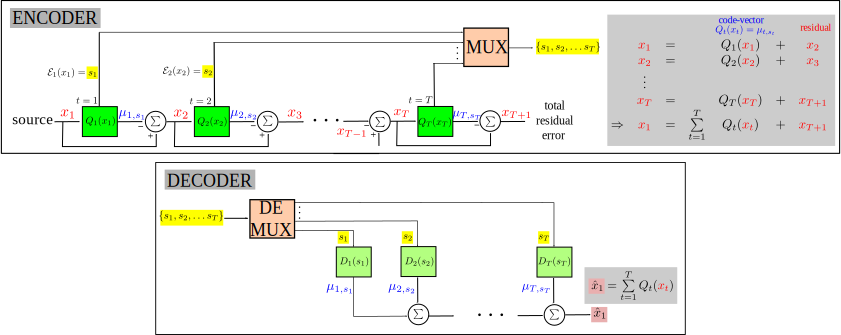
\includegraphics[width=1\textwidth]{thesis/RVQ_blockDiagram.pdf}
	\caption{RVQ: block diagram}
	\label{fig:RVQ_block_diagram}
\end{figure}

An RVQ is different from a traditional VQ in the sense that it partitions the input space $R^D$ into $M$ cells.  The residual space, also in $R^D$, is then partitioned again into $M$ cells.  This process is repeated $T$ times.  The advantage of this approach is that in obtaining $M^T$ partitions, we need to run our partitioning algorithm $T$ times and generate $M$ partitions at each stage.  In traditional VQ, the partitioning algorithm would run once but have to create $M^T$ partitions.  For the binary case (two code-vectors per stage, $M=2$) and a total of 8 stages ($T$=8), RVQ only requires 16 searches.  In $ESVQ$, this would require 256.  The exponential complexity is reduced to linear complexity.  Moreover, even the distortion of an ESVQ can be attained.  In general, all structurally constrained quantizers cannot provide performance as good as ESVQ.  However, since they are able to more efficiently implement codes, larger and larger vector sizes can be used, and if carefully designed, can achieve better performance that ESVQ \cite{1996_JNL_AdvancesRVQ_Barnes}.

\begin{figure}[ht]
	\centering	
	\subfigure[]
	{
		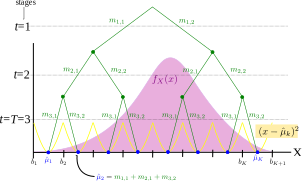
\includegraphics[width=0.65\textwidth]{thesis/RVQ_graphicalReconstruction.pdf}
		\label{fig:MTT_codebooks}	
	}
	\subfigure[]
	{
		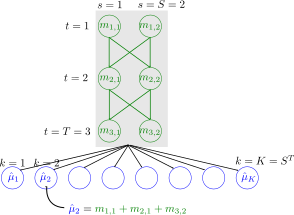
\includegraphics[width=0.65\textwidth]{thesis/RVQ_trellis.pdf}
		\label{fig:MTT_reconstruction}	
	}
	\caption{RVQ $\sigma$-tree, $T$=3, $S=2$, two alternate representations} 
	\label{fig:RVQ_sigma_tree}				
\end{figure}


%=======================
\subsection{Encoder}
%=======================
A vector quantizer with a direct sum codebook,

\begin{itemize}
\item is the source coding dual of a $\sigma$-tree structure \cite{1993_sigmaTrees_Barnes}, and
\item its design is the covering design problem
\end{itemize}

Since the dual of the covering problem is the packing problem \cite{BOOK_spheres_Conway}, it is shown in \cite{1993_sigmaTrees_Barnes} that $\sigma$-tree structures exist that provide good packing.  The design of RVQ direct sum codebooks is therefore studied in the context of $\sigma$-trees.

The set $\mathcal{S}$ of $K$ leaf nodes of a $T$-level $M$-ary $\sigma$-tree is the set of $M^T$ direct sums of $T$ vectors in $R^D$, one vector per level $t$ being picked from a \emph{constituent set} $G_t = \{m_{t,m} \in R^D \ | m=1, 2, \ldots M\}$ \cite{2002_JNL_SigmaTrees_Barnes},

\begin{equation}
\mathcal{S} = \{\hat{\mu}^{(k)} \in R^D \ | \ \hat{\mu}_k = \sum\limits_{t=1}^T m_t^{(k)}, k=1, 2, \ldots, K=M^T\}
\end{equation}

An example 3-level binary $\sigma$ tree is given in Figure~\ref{fig:RVQ_sigma_tree}.  The RVQ encoder can be designed in two major phases which are explained below and illustrated in Figure~\ref{fig:RVQ_encoder_flowDiagram}. 
 


 

\begin{figure}[ht]
\centering
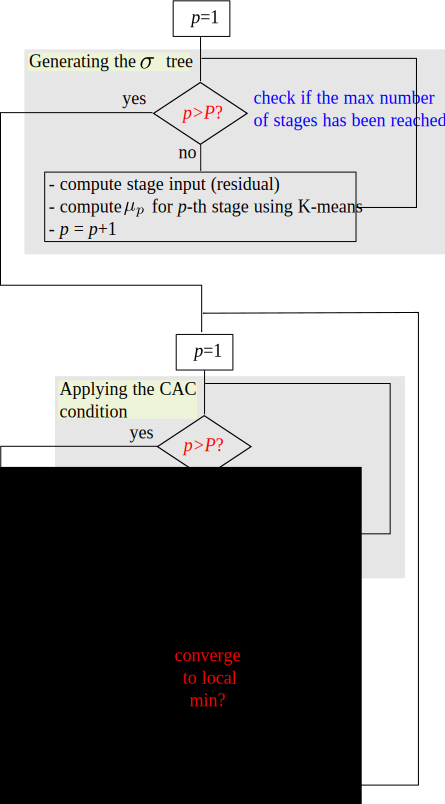
\includegraphics[height=0.6\textheight]{thesis/RVQ_encoder_flowDiagram.pdf}
\caption{Encoder flow diagram, generating codebooks $\Phi$}
\label{fig:RVQ_encoder_flowDiagram}
\end{figure}


\begin{enumerate}
\item \underline{Generating the $\sigma$ tree}.  The first design step is to generate the RVQ $\sigma$-tree by repeated application of the K-means algorithm to every stage in the following manner:  
\begin{enumerate}
\item \underline{First stage}. As in the K-means algorithm, standard practice is to generate several arbitrary partitionings and to retain the partition that results in least error as given by Equation~\ref{Eq:computingClusterCentroids}.  The objective function for the discrete case is,

\begin{equation}
\label{Eq:KmeansError}
e = \KmeansError
\end{equation}

The means of this partitioned data constitute the first stage codevectors.  In effect, this step generates $S$ stage codevectors, where typically, $S << K$.  For instance, if $K=16$ clusters are desired in ESVQ, RVQ can attain that many clusters with say $T=4$ stages and $S=2$ codevectors per stage.  Notice that in this equation, it is implicit that the partitions are known.  The outer summation that sums over the $K$ clusters is what makes this an NP hard problem, otherwise this would be a standard least squares problem.  Once the partitions are fixed, this can be solved as a standard least squares problem by setting the derivatives equal to 0.  

\begin{align}
\frac{\partial{e}}{\partial{\mu_k}} &= 0\notag\\
\KmeansInnerSum 2 \KmeansInner &= 0\notag\\
\KmeansInnerSum x_i - \KmeansSum \mu_k &= 0\notag\\
\KmeansInnerSum x_i - N_k \mu_k &= 0\notag\\
\mu_k &= \frac{\KmeansInnerSum x_i}{N_k}
\label{Eq:computingClusterCentroids}
\end{align}

In the equation above, $\mu_k$ is the cluster centroid for the $k$-th partition $\mathcal{K}_k$.  Once the $K$ cluster centroids have been computed, the data is repartitioned.  In other words, data points are mapped to the nearest new cluster centroids.  The cluster centroids are recomputed using Equation~\ref{Eq:computingClusterCentroids}.  This process of partitioning followed by centroid computation followed by repartitioning followed by centroid computation is repeated till the centroids converge.

\item \underline{Generating residual stages}.  In the step above, stage codevectors are subtracted from the data points that map to them.  This step generates a new set of data points, the first stage \emph{residual} data points.  The data at the output of stage $t$ is called the $t$-th residual data.  This causes each cluster in the first stage to be centered around the origin and also causes each data point to move closer to the origin.  These residual data points are now input into the K-means algorithm which generates a new set of partitions and new cluster centroids.  Using the same procedure discussed earlier, second stage residuals are generated and input to the third stage.  This process is repeated till the desired number of stages.  This Markovian style design process generates the initial RVQ $\sigma$-tree trellis.  
\end{enumerate}
\item \underline{Applying the CAC condition}.  The above step generates cluster centroids that are locally optimal at every stage.  Morever, the design of each stage depends on the previous or causal stage designs but does not depend on subsequent or anti-casual stage designs.   This can lead to a propagation of reconstruction error.  No optimality claims can be made regarding this design process.  An attempt to address this is a joint design strategy, also known as the Causal Anti-causal (CAC) condition.  This is explained next.
\end{enumerate}

\begin{figure}
\center
\includegraphics[width=0.5\textwidth]{thesis/RVQ_CAC_toyExample2_2x2.pdf}
\caption{2x2 RVQ example}
\label{fig:Figure1}
\end{figure}





\subsubsection{Causal Anti-causal condition}
%---------------------------------------------------
To understand CAC, it is beneficial to first introduce some notation:

\begin{itemize}
\item \emph{Path}.  A finite directed path through the RVQ $\sigma$-tree has as its vertices one stage codevector from every stage.  For $T$ stages and $S$ codevectors per stage, there are a total of $K = S^T$ possible paths.
\item \emph{Stage codevector}.  A stage codevector $m_{t, s}$ is the $s$-th codevector at the $t$-th stage.  An alternate notation used is $m^{(k)}_t$ which denotes the stage codevector at the $t$-th stage for the $k$-th path.
\item \emph{Optimal reconstruction}.  There are $K=S^T$ possible paths through the RVQ $\sigma$-tree.  Each data point $x_i$ propagates through the $\sigma$-tree on one of these $K$ paths.  If $x_i \mapsto \mathcal{K}_k$, then for optimal reconstruction, the following condition must hold true,

\begin{equation*}
\RVQunit = 0, \ \ \forall x_i \mapsto \mathcal{K}_k, \ \ i =1, 2, \ldots N\\
\end{equation*}

where $m^{(k)}_t$ is the stage codevector at the $t$-th stage of the $k$-th path through the $\sigma$-tree.  The above condition shows that

\begin{itemize} 
\item There are at most $K=S^T$ distinct data points that can result in 0 reconstruction error, irrespective of the dimensionality $D$ of the data. 
\item The non-Markovian reconstruction function produces a Direct Sum Successive Approximation (DSSA) of the input.
\end{itemize}\item \emph{Equivalent codevector}.  For every path through the RVQ $\sigma$-tree, we have an equivalent codevector $\hat{\mu}^{(k)}$ given by,
\begin{equation}
\hat{\mu}^{(k)} = \RVQequivalentCodevector, \ \ \ k=\{1, 2, \ldots, K\}
\end{equation}
In general, the $K$ equivalent codevectors and the accompanying $K$ partitions will approximate the $K$ cluster centroids and $K$ partitions produced by ESVQ.  The equivalent codevector can also be written as,
\begin{equation}
\label{Eq:RVQequivalentCodevectorBroken}
\hat{\mu}^{(k)} = \RVQequivalentCodevectorBroken
\end{equation}
\item \emph{RVQ objective function}.  The ESVQ objective function in Equation~\ref{Eq:KmeansError} can now be re-written in terms of the equivalent codevectors as 
\begin{equation}
e = \RVQerror
\end{equation}
\end{itemize}

Substituting for the equivalent codevector from Equation~\ref{Eq:RVQequivalentCodevectorBroken} gives

\begin{equation}
e=\KmeansSum{\bigg[\RVQmultipleKmeans\bigg]}^2, \ \ \tau=\{1, 2, \ldots T\}
\label{Eq:RVQmultipleKmeans}
\end{equation}

This equation states that for RVQ, the original objective function can be written as a series of coupled K-means equations, one equation per stage.    
 
\begin{align}
e&= \KmeansSum{\bigg[\RVQmultipleKmeansone\bigg]}^2, \ \ \tau=1\notag\\
&= \KmeansSum{\bigg[\RVQmultipleKmeanstwo\bigg]}^2, \ \ \tau=2\notag\\
&\ \ \ \  \ \ \ \vdots\notag\\
&=\KmeansSum{\bigg[\RVQmultipleKmeansT\bigg]}^2, \ \ \tau=T
\end{align}

Equation~\ref{Eq:RVQmultipleKmeans} can now be regrouped as,

\begin{align}
\label{Eq:RVQmeans}
e&= \KmeansSum{\bigg[\RVQmultipleKmeansonealternate\bigg]}^2, \ \ \tau=\{1, 2, \ldots T\}\notag\\
&={\RVQerroralternate}, \ \ \tau=\{1, 2, \ldots T\}
\end{align}

where $g_i$ is the \emph{graft residual} and is formed using the following steps,

\begin{itemize}
\item \emph{List all reconstruction stage codevectors in path}.  For a data point $x_i$, list all stage codevectors that are used to reconstruct it
\item \emph{Find graft residual at stage $\tau$}.  Subtract all stage codevectors in above step from $x_i$ except the stage codevector at the $\tau$-th stage  
 \end{itemize}

Equation~\ref{Eq:RVQmeans} is now quite clearly a K-means objective function for the $\tau$-th stage.  Here, $m_{\tau}^{(k)}$ is a single codevector at the $\tau$-th stage even though it has a superscript $k$ which tends to indicate that it might correspond to several codevectors.  The superscript $k$ refers to the fact that there are $K$ possible paths, but for a particular $g_i$, we choose the $m_{\tau}^{(k)}$ that lies in the reconstruction path of the corresponding $x_i$.  We can therefore rewrite Equation~\ref{Eq:RVQmeans} as,

\begin{equation}
e = \RVQOuterSum\RVQInnerSum\RVQinneralternatealternate
\end{equation} 

Now, to compute a particular stage codevector $m_{\tau, s}$, we use the standard GLA algorithm as in Equation~\ref{Eq:computingClusterCentroids} to get

\begin{equation}
m_{\tau, s} = \frac{\RVQInnerSum g_i}{N_{g_i \mapsto m_{\tau, s}}}
\label{Eq:finalCAC}
\end{equation}

\begin{figure}[ht]
\centering
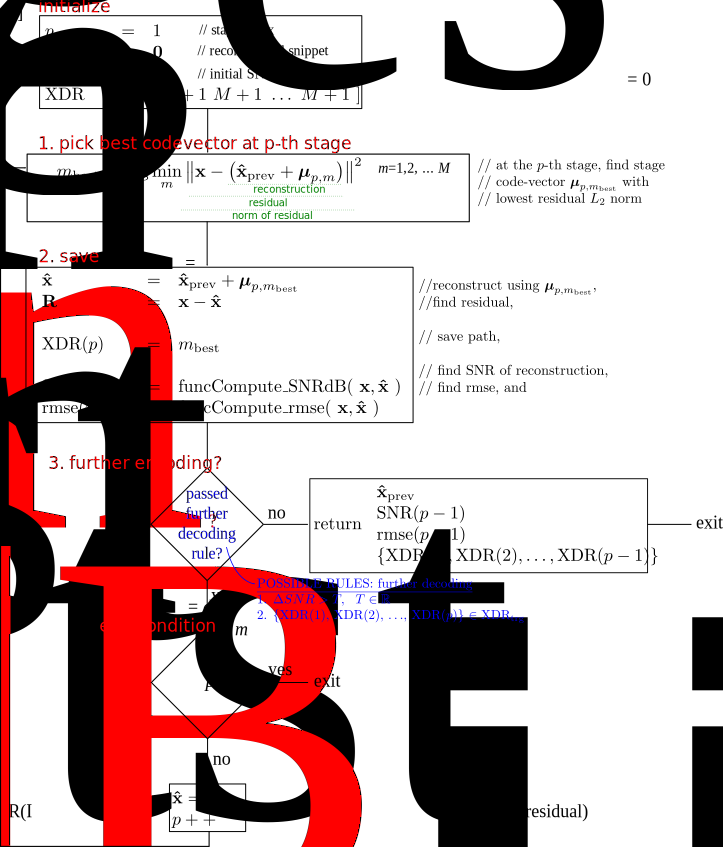
\includegraphics[height=0.6\textheight]{thesis/RVQ_explorer_flowDiagram.pdf}
\caption{Decoder flow diagram}
\label{fig:RVQ_decoderFlowDiagram}
\end{figure}


Equation~\ref{Eq:finalCAC} can now be used to compute the $S$ stage codevectors at the $\tau$-th stage.  $N_{g_i \mapsto m_{\tau, s}}$ is the number of graft residuals $g_i$ whose corresponding data points $x_i$ contain $m_{\tau, s}$ in their reconstruction path.  Recall that in ordinary K-means, computation of the centroids is followed by a repartitioning which is followed by a centroid computation and so on.  This process is repeated till convergence.  However, in this case of coupled K-means, two issues arise:

\begin{itemize}
\item repartitioning affects all stages.  
\item Moreover, recomputing the centroids for one stage changes the graft residuals for all other stages, since each graft residual depends on $S-1$ stage codevectors.  
\end{itemize}

Since RVQ update strategies are not the focus of this research, the reader is referred to  \cite{1996_JNL_AdvancesRVQ_Barnes} for more details.  The result of these steps is an RVQ codebook with $K$ codevectors,

\begin{equation}
\mathcal{M} = \{\hat{\mu}_1, \hat{\mu}_2, \ldots, \hat{\mu}_K\}
\end{equation}

Figure~\ref{fig:Figure1} shows a simple example of a 2x2 RVQ with 4 input data points.  The error is given by



\begin{equation}
\begin{array}{lllll}
e &=& \KmeansError \\
&=& {(x_1 - a - c)}^2 + {(x_2- a - d)}^2 + {(x_3 - b - c)}^2 + {(x_4 - b - d)}^2\\
&=& {e_1}^2 + {e_2}^2 + {e_3}^2 + {e_4}^2
\end{array}
\end{equation}

Applying the CAC condition to optimize stage 1, we get the following equations by grouping all input data points with stage codevectors that do not belong to stage 1,

\begin{equation}
\begin{array}{lllll}
e &=& {((x_1 - c) - a)}^2 + {((x_2- d) - a)}^2 + {((x_3 - c) - b)}^2 + {((x_4 - d) - b)}^2
\end{array}
\label{Eqn:2x2RVQ_stage1}
\end{equation}

And similarly, to optimize stage 2, we get,

\begin{equation}
\begin{array}{lllll}
e &=& {((x_1 - a) - c)}^2 + {((x_2- a) - d)}^2 + {((x_3 - b) - c)}^2 + {((x_4 - b) - d)}^2
\end{array}
\label{Eqn:2x2RVQ_stage2}
\end{equation}

which leads to the optimal stage codevectors,

\begin{equation}
\begin{array}{lllll}
a = \frac{(x_1 - c) + (x_2 - d)}{2}\\
b = \frac{(x_3 - c) + (x_4 - d)}{2}\\
c = \frac{(x_1 - a) + (x_3 - b)}{2}\\
d = \frac{(x_2 - a) + (x_4 - b)}{2}\\
\end{array}
\end{equation}

%=======================
\subsection{Decoder}
%=======================
The decoder has a DSSA (direct sum successive approximation) structure.  In other words, at the first stage, the best first stage codevector in the $L_2$ norm sense is picked.  This codevector is subtracted from the input signal to form a first stage residual signal.  This signal is fed as input to the second stage where again the best second stage codevector in the $L_2$ norm sense is picked.  The residual from this stage is fed as input to the third stage.  This process is repeated for all $T$ stages.  The final residual output from the $T$-th stage is the error signal.  The reconstructed output signal is a sum of the best codevectors at every stage.  This process is shown in detail in Figure~\ref{fig:RVQ_decoderFlowDiagram}.  In this diagram, the reconstructed signal is first initialized to the zero vector.  At every stage, the SNR of the reconstructed signal is computed.  The process of decoding is stopped when either the maximum number of stages have been achieved or if the SNR does not increase at any stage.  In other words, a monotonic SNR increase condition is imposed.  The computational complexity of this decoding process is $O(N)$.  


%=======================
\subsection{Toy example}
%=======================


%\mbox{testing method 1} &&& \mbox{maximize log likelihood}\\
%c^*_b&=& \mbox{arg}\max\limits_c & \log p(\mathcal{C}_c | \mathbf{Y})\\
%&=& \mbox{arg}\max\limits_c & \log p(\mathbf{Y} | \mathcal{C}_c)\\
%&=& \mbox{arg}\max\limits_c & \log p(Y_1 = \mathbf{b}_n(1), Y_2 = \mathbf{b}_n(2),  \ldots , Y_T = \mathbf{b}_n(T) | \mathcal{C}_c)\\
%&=& \mbox{arg}\max\limits_c & \sum\limits_{t=1}^{T} \log p \bigg(Y_t | Y_{t-1}, \mathcal{C}_c \bigg) \\ \\ \\ \\
%\mbox{testing method 2} &&& \mbox{maximize  KL divergence (relative entropy)}\\
%c^*_{r,c}&=& \mbox{arg}\max\limits_c & \sum \log \frac{p(\mathbf{X}|\mathcal{C}_c)}{p(\mathbf{Y})}p(\mathbf{X}|\mathcal{C}_c) \\
%
%&=& \mbox{arg}\max\limits_c & \bigg[\log p \bigg(\mathcal{C}_c|X_1=\mathbf{b}_{r,c}(1) \bigg) + \sum\limits_{t=2}^{T} \log p \bigg(\mathcal{C}_c | X_t = \mathbf{b}_{m,n}(t), X_{t-1} = \mathbf{b}_{r,c}(t-1) \bigg) - \\
%
%
%&&& \log p \bigg(Y_1=\mathbf{b}_{r,c}(1) \bigg) + \sum\limits_{t=2}^{T} \log p \bigg(Y_t = \mathbf{b}_{r,c}(t), Y_{t-1} = \mathbf{b}_{r,c}(a-1) \bigg) \bigg]p(X_1|\mathcal{C}_c)p(X_2|X_1, \mathcal{C}_c)p(X_3|X_2, \mathcal{C}_c) \ldots p(X_T|X_{T-1}, \mathcal{C}_c)
%\\ \\ \\ \\
%
%
%
%\mbox{testing method 3} &&& \mbox{maximize mutual information}\\
%p(\mathbf{X};\mathbf{Y}) &=&& H(\mathbf{X}) - H(\mathbf{X|Y})
%\end{array}
%\end{equation}

%$
%\mbox{- for an RVQ with $T$ stages, an SoC is a $T$-tuple containing reconstruction indeces for a block of source symbols} \\
%\mbox{- during training, each reconstruction index takes on values from the alphabet } \Phi_{trg}\\
%\mbox{- during testing, each reconstruction index takes on values from the alphabet } \Phi_{tst}\\
%\mbox{- for stage $t$, i.e. the $t$-th component of the SoC descriptor, the reconstruction index is the stage-codevector index $m$ for that stage as long as $m \leq M$} \\
%\mbox{- during testing, $M+1$ and $M+2$ are used as fillers to make sure that the test SoC has length $T$}
%$







%Another question here concerns the optimality of RVQ.  An RVQ is said to be \emph{jointly optimal} if a local or global minimum value of the average distortion $\mathcal{D}(E,D) = E[m(X_1, D(E(X_1)))]$ is achieved.  Here, $E$ is the encoder, $D$ is the decoder, $m(.,.)$ is a distortion metric, and $E[.]$ is the expectation operator.  The necessary condition for joint decoder optimality is that the code-vectors $y_p(i)$  of the $p$-th stage must satisfy the following condition:
%
%\begin{equation}
%\mathcal{D}=\frac{\partial D}{\partial y_p(i)}=0
%\end{equation}
%
%This condition is satisfied when the stage code-vectors are centroids of residuals formed from the encoding decisions of both \emph{causal} and \emph{anticausal} stages \cite{1995_JNL_OptimalityRVQ_Kossentini}.  On the other hand, if only causal stages are considered, then satisfying the condition above will help achieve \emph{sequential} optimality.  For the encoder case, it is not possible to design optimal stages.  Instead an overall global unconstrained encoder is designed, and then individual encoder stages are designed using nearest neighbor rules that try to match the performance of the global encoder.
%
%A final note is that due to the multiple stages of RVQ, it is possible to design with few code-vectors per stage.  This can be useful if the training data is limited, since this would necessitate the use of small stage-codebook sizes \cite{1996_JNL_AdvancesRVQ_Barnes}.


%Channel coding is sphere packing and rate distortion coding is sphere covering \cite{2006_BOOK_InformationTheory_Cover}. 


